\chapter{Ergebnisse/ Numerische Experimente}
Im Folgenden werden einige simple Beispiele betrachtet,
welche mit dem zur Arbeit begleitenden Programm berechnet wurden.
Die Ergebnisse werden anschließend mit Werten aus
einem professionellen Programm verglichen,
um die qualitative Korrektheit der Implementierung zu bestätigen.
\section{Aufbau}
Wir schauen uns die folgenden Moleküle an:
\begin{enumerate}
    \item Heliumhydridion (HeH$^+$)
    \item Wasser (H$_2$O)
    \item Ammoniak (NH$_3$)
    \item Methan (CH$_4$)
\end{enumerate}
\begin{figure}[h]
    \centering
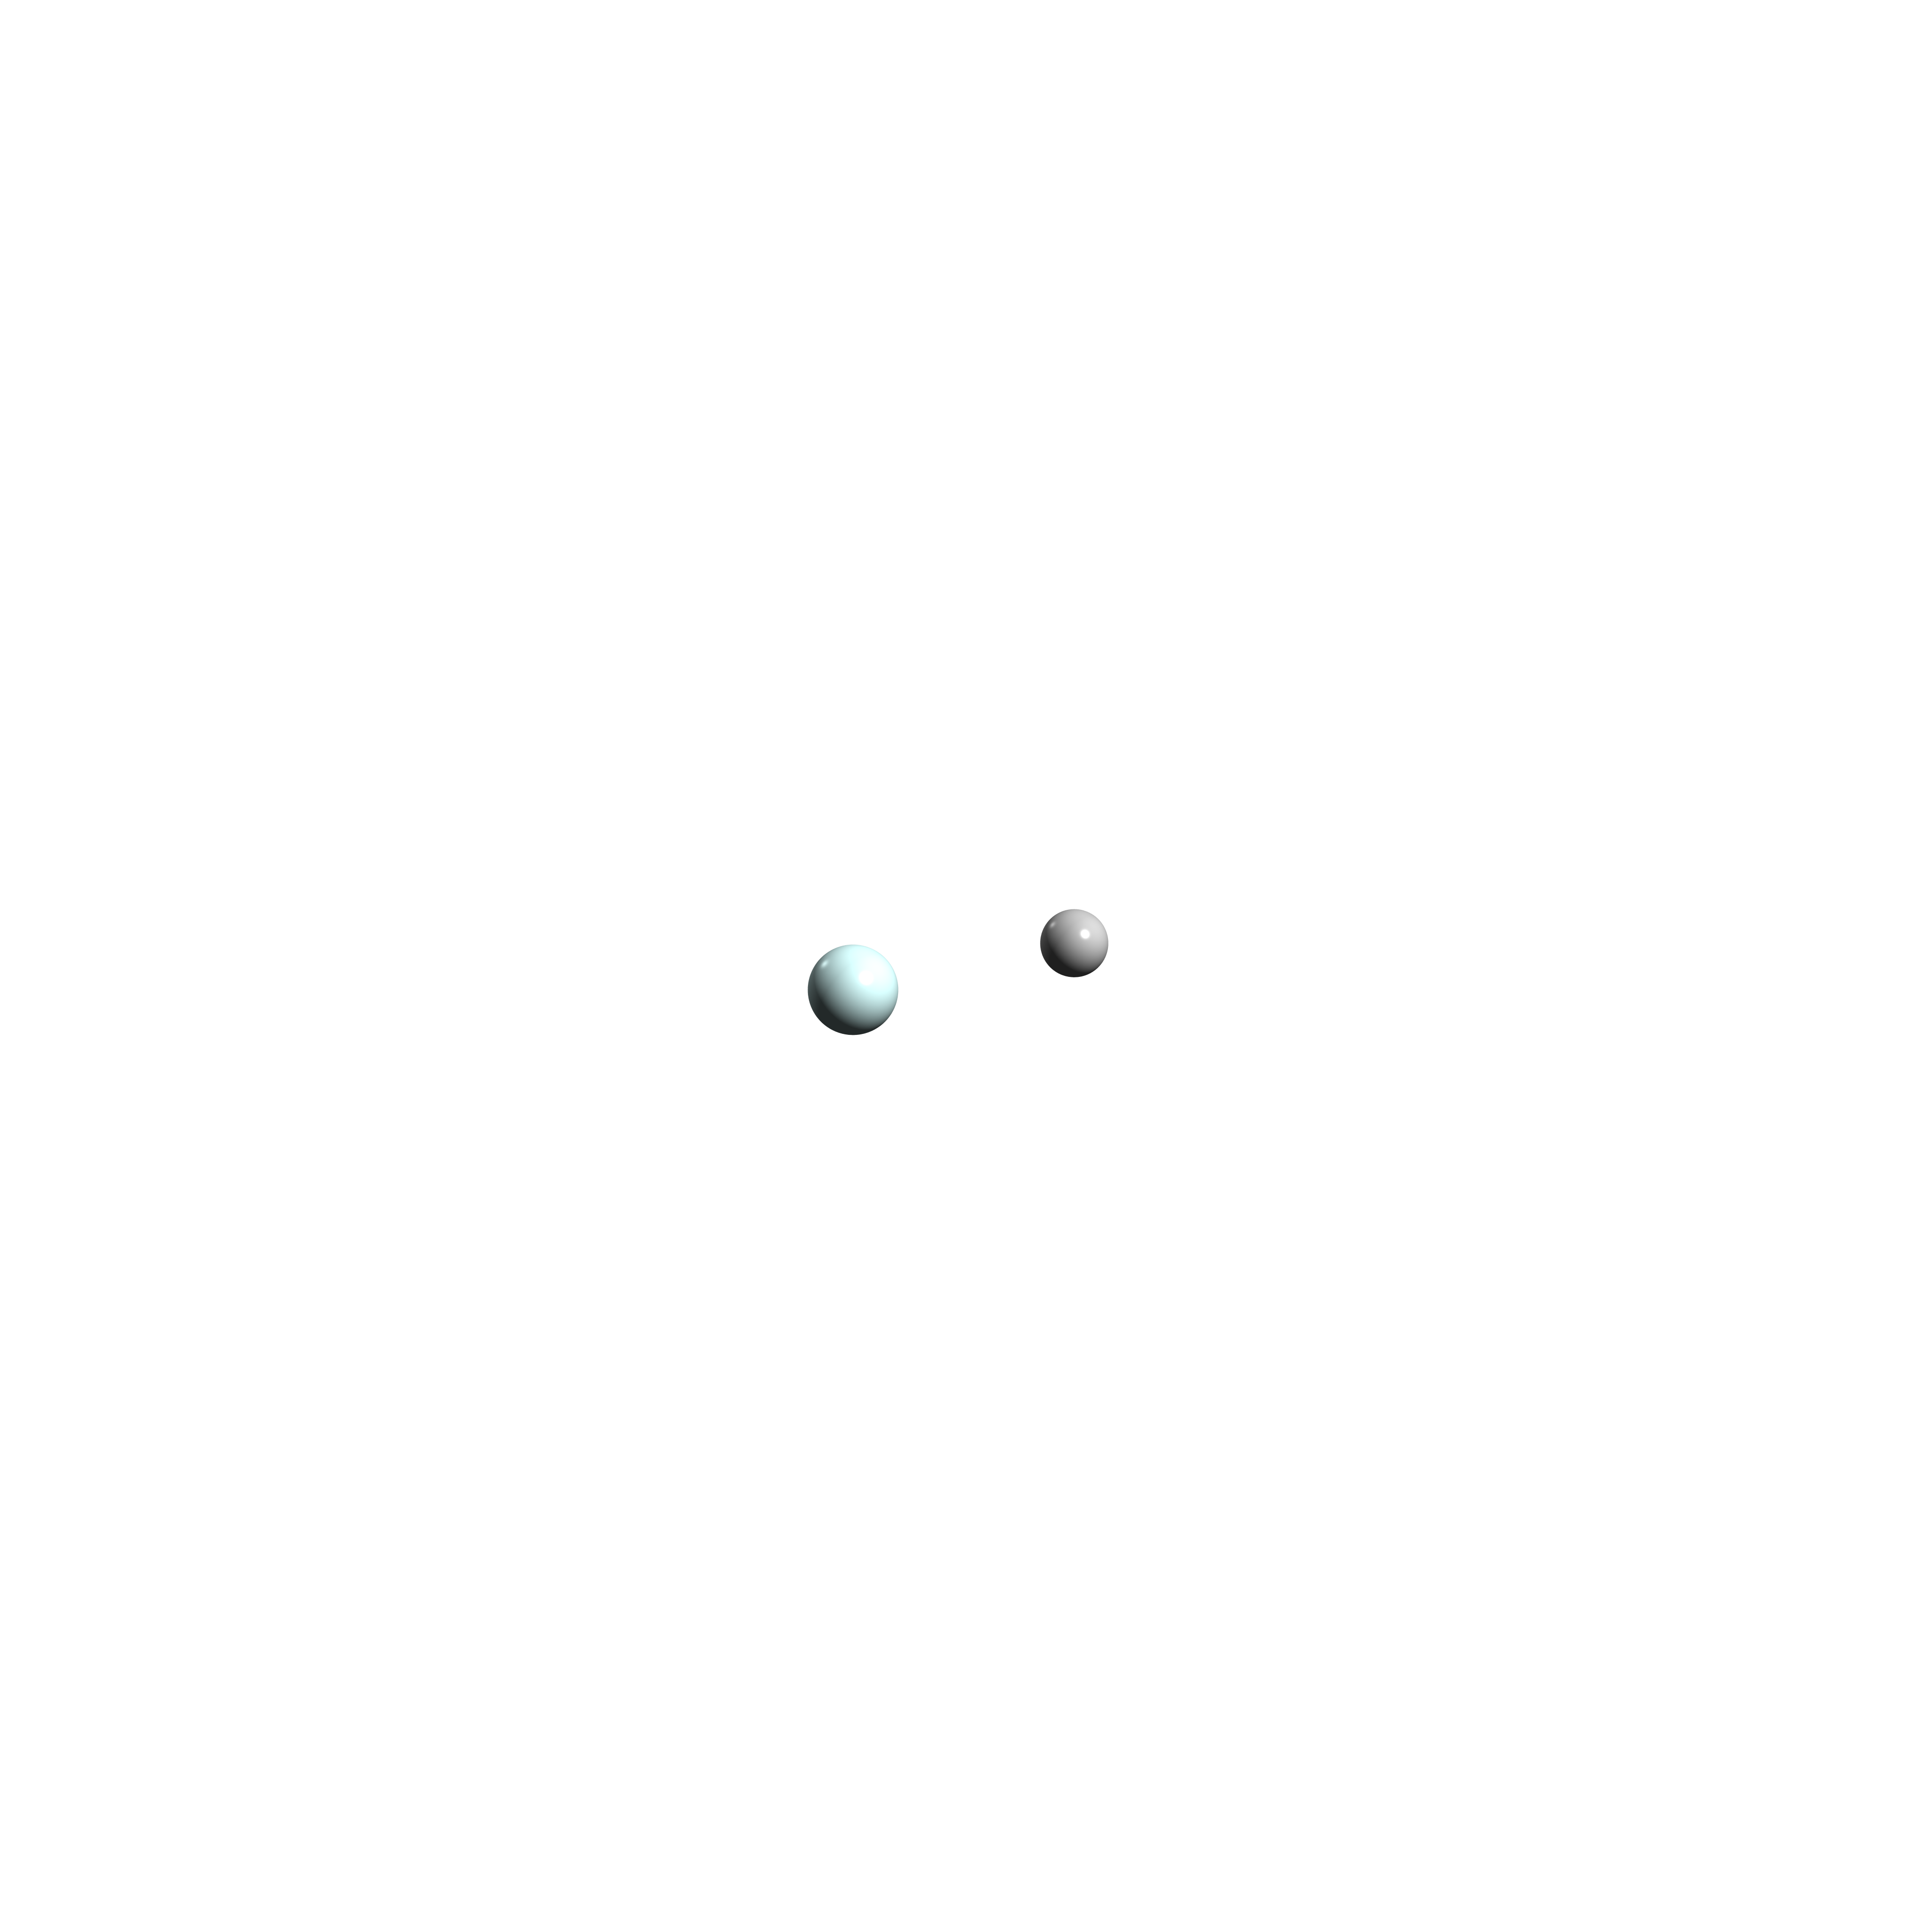
\includegraphics[trim=1400 1400 1400 1400, clip, width=0.24\textwidth]{res/HeH/heh_w.png}
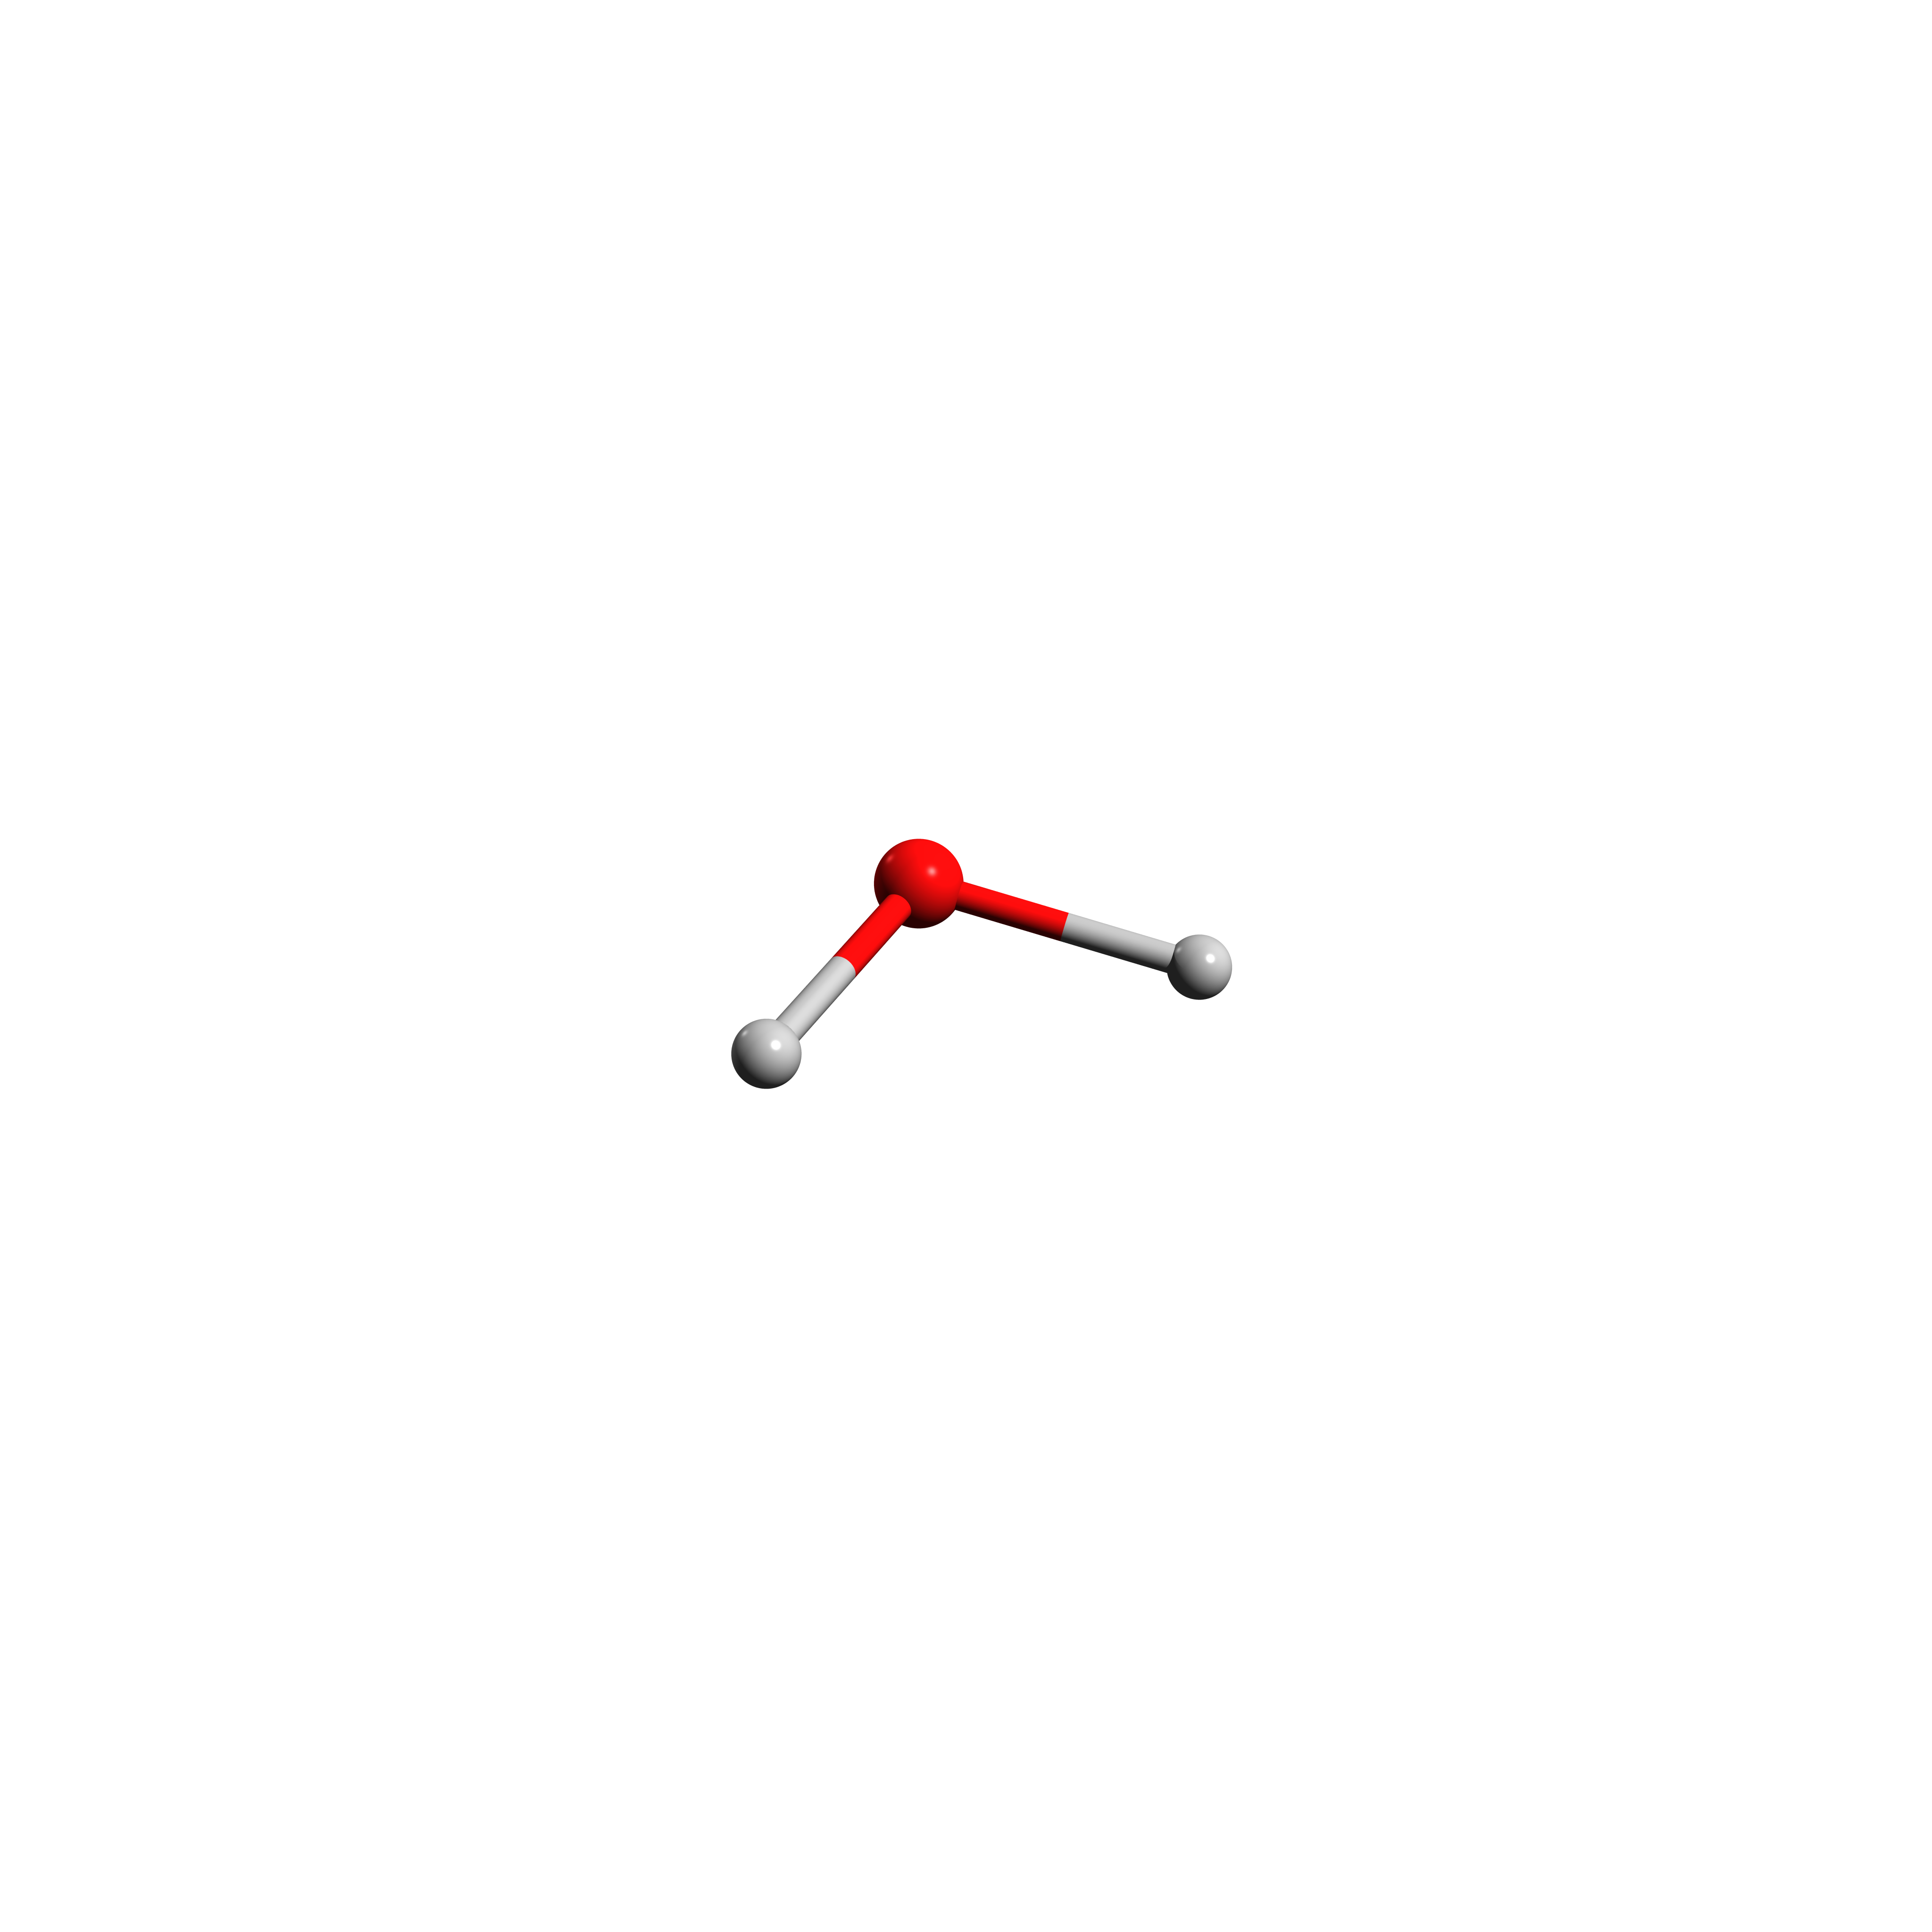
\includegraphics[trim=1400 1400 1400 1400, clip, width=0.24\textwidth]{res/H2O/h2o.png}
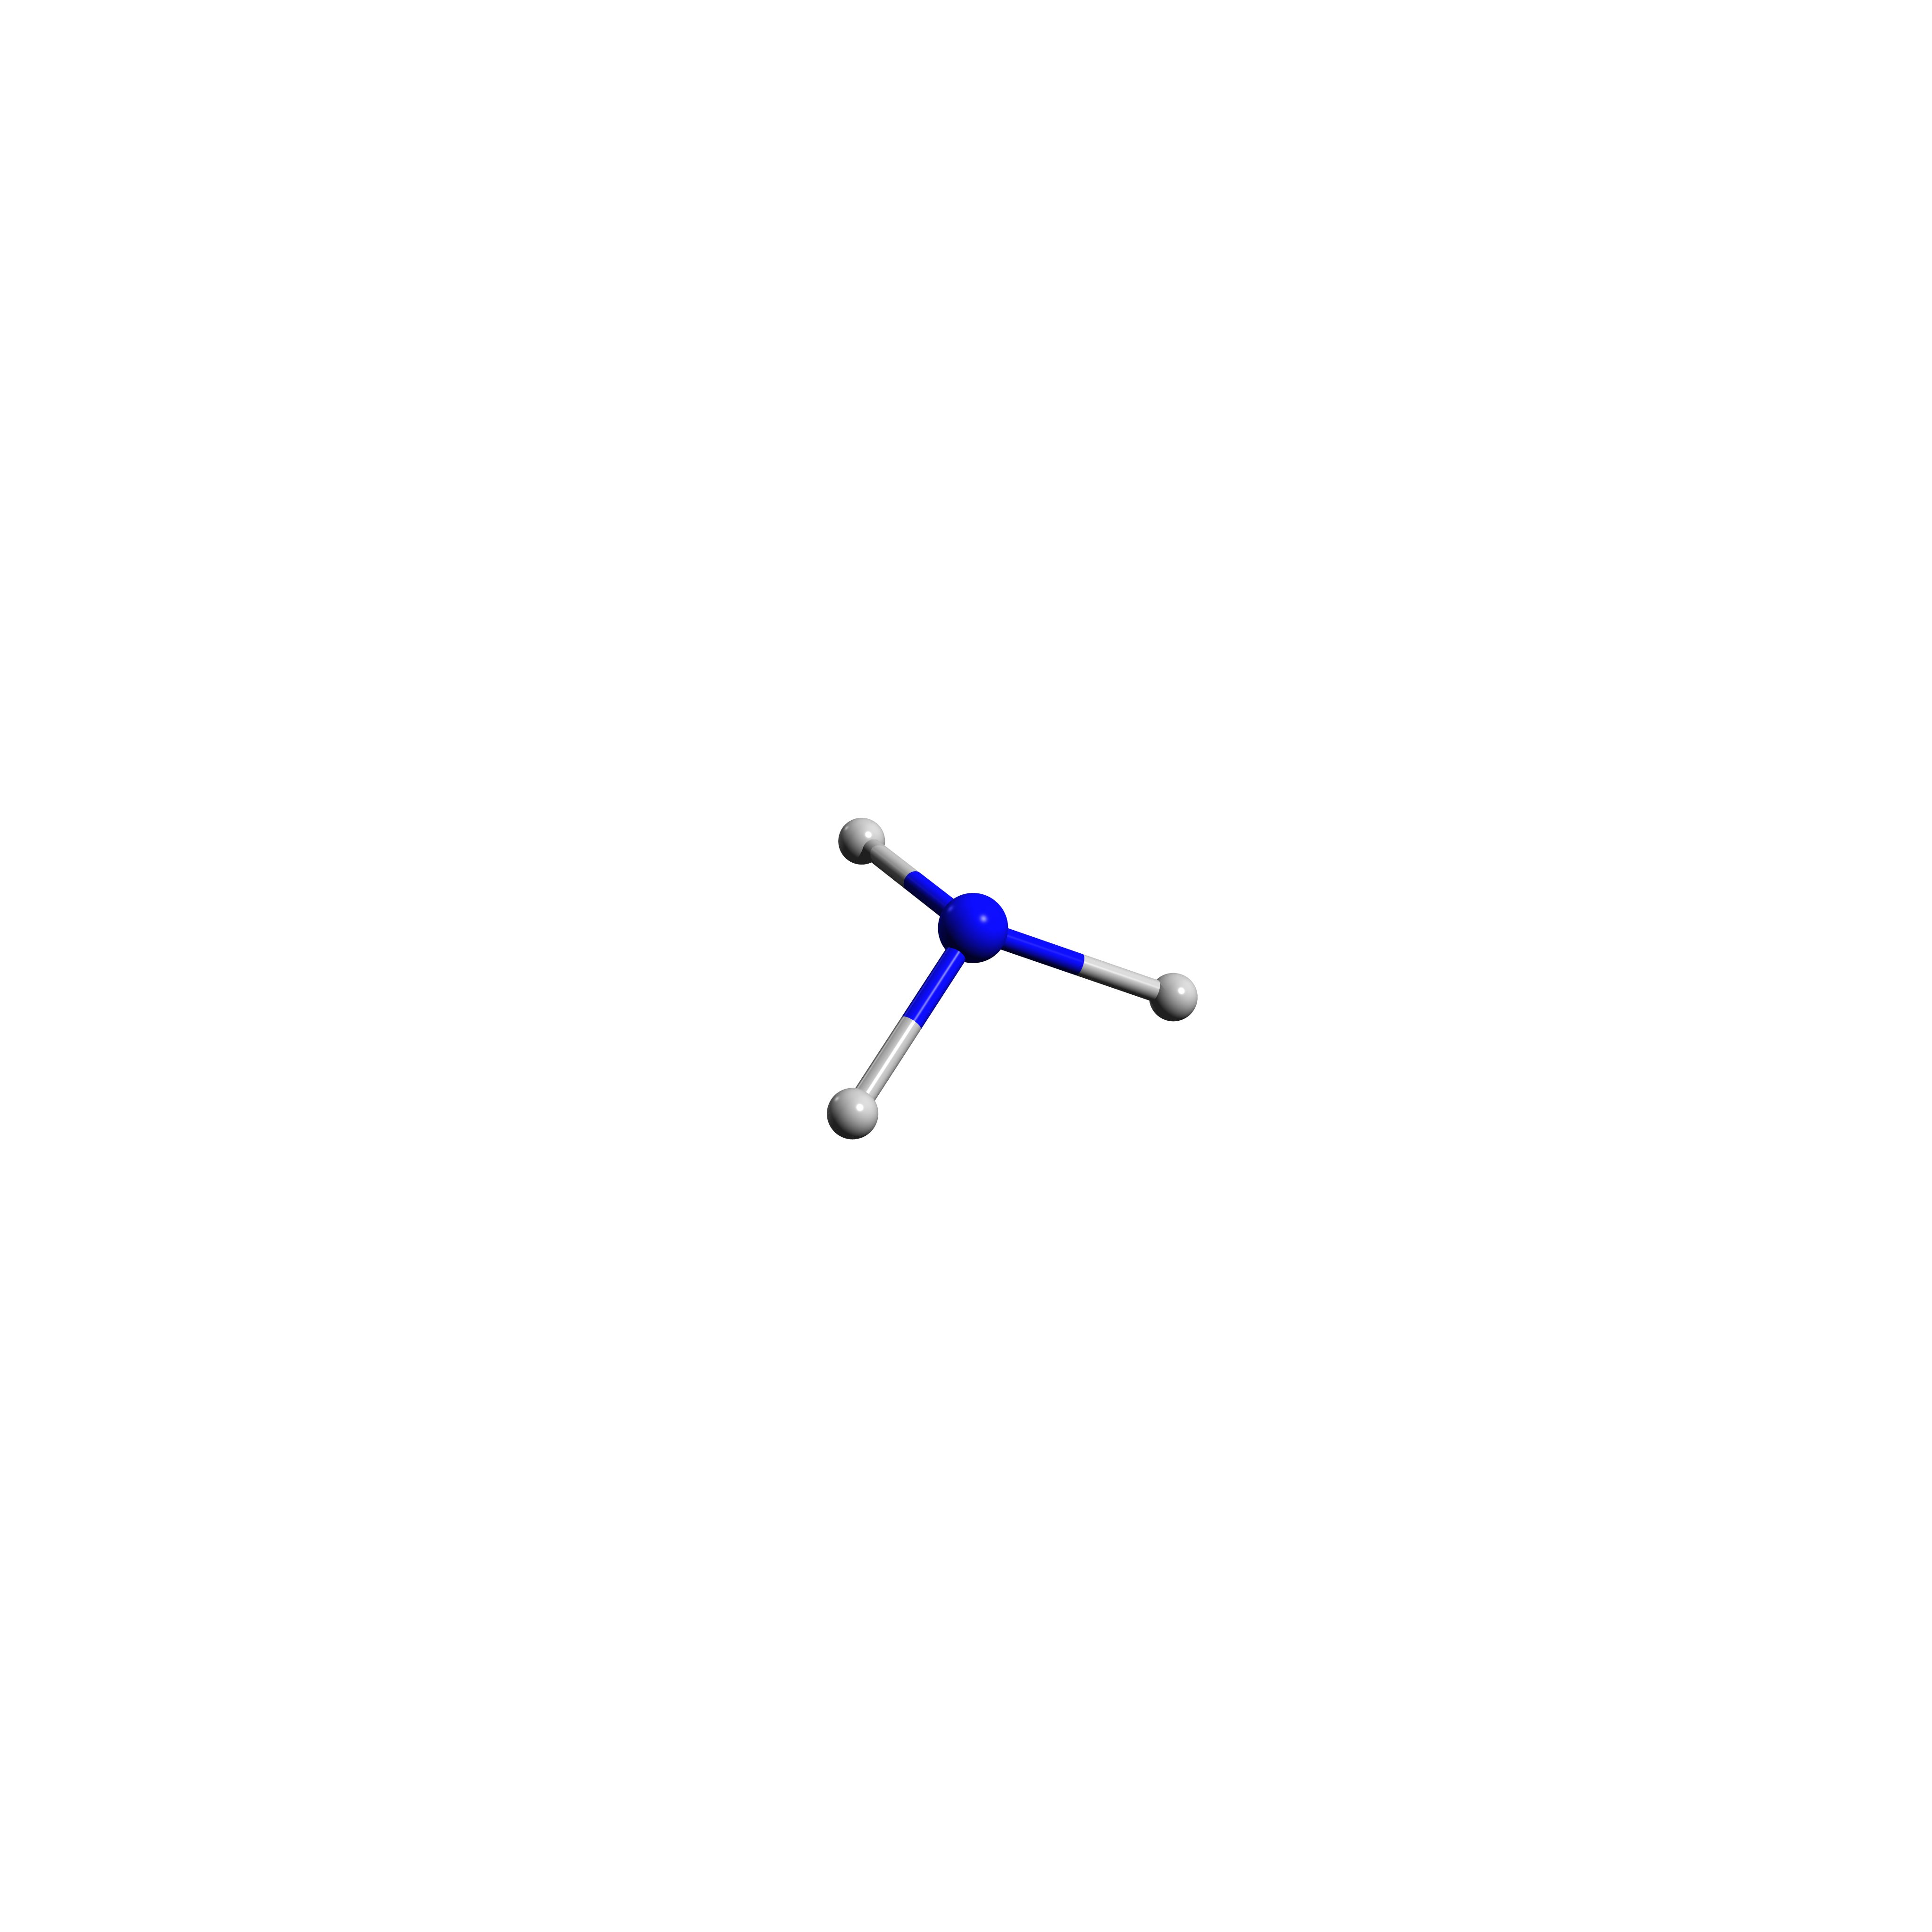
\includegraphics[trim=1400 1400 1400 1400, clip, width=0.24\textwidth]{res/NH3/nh3_d.png}
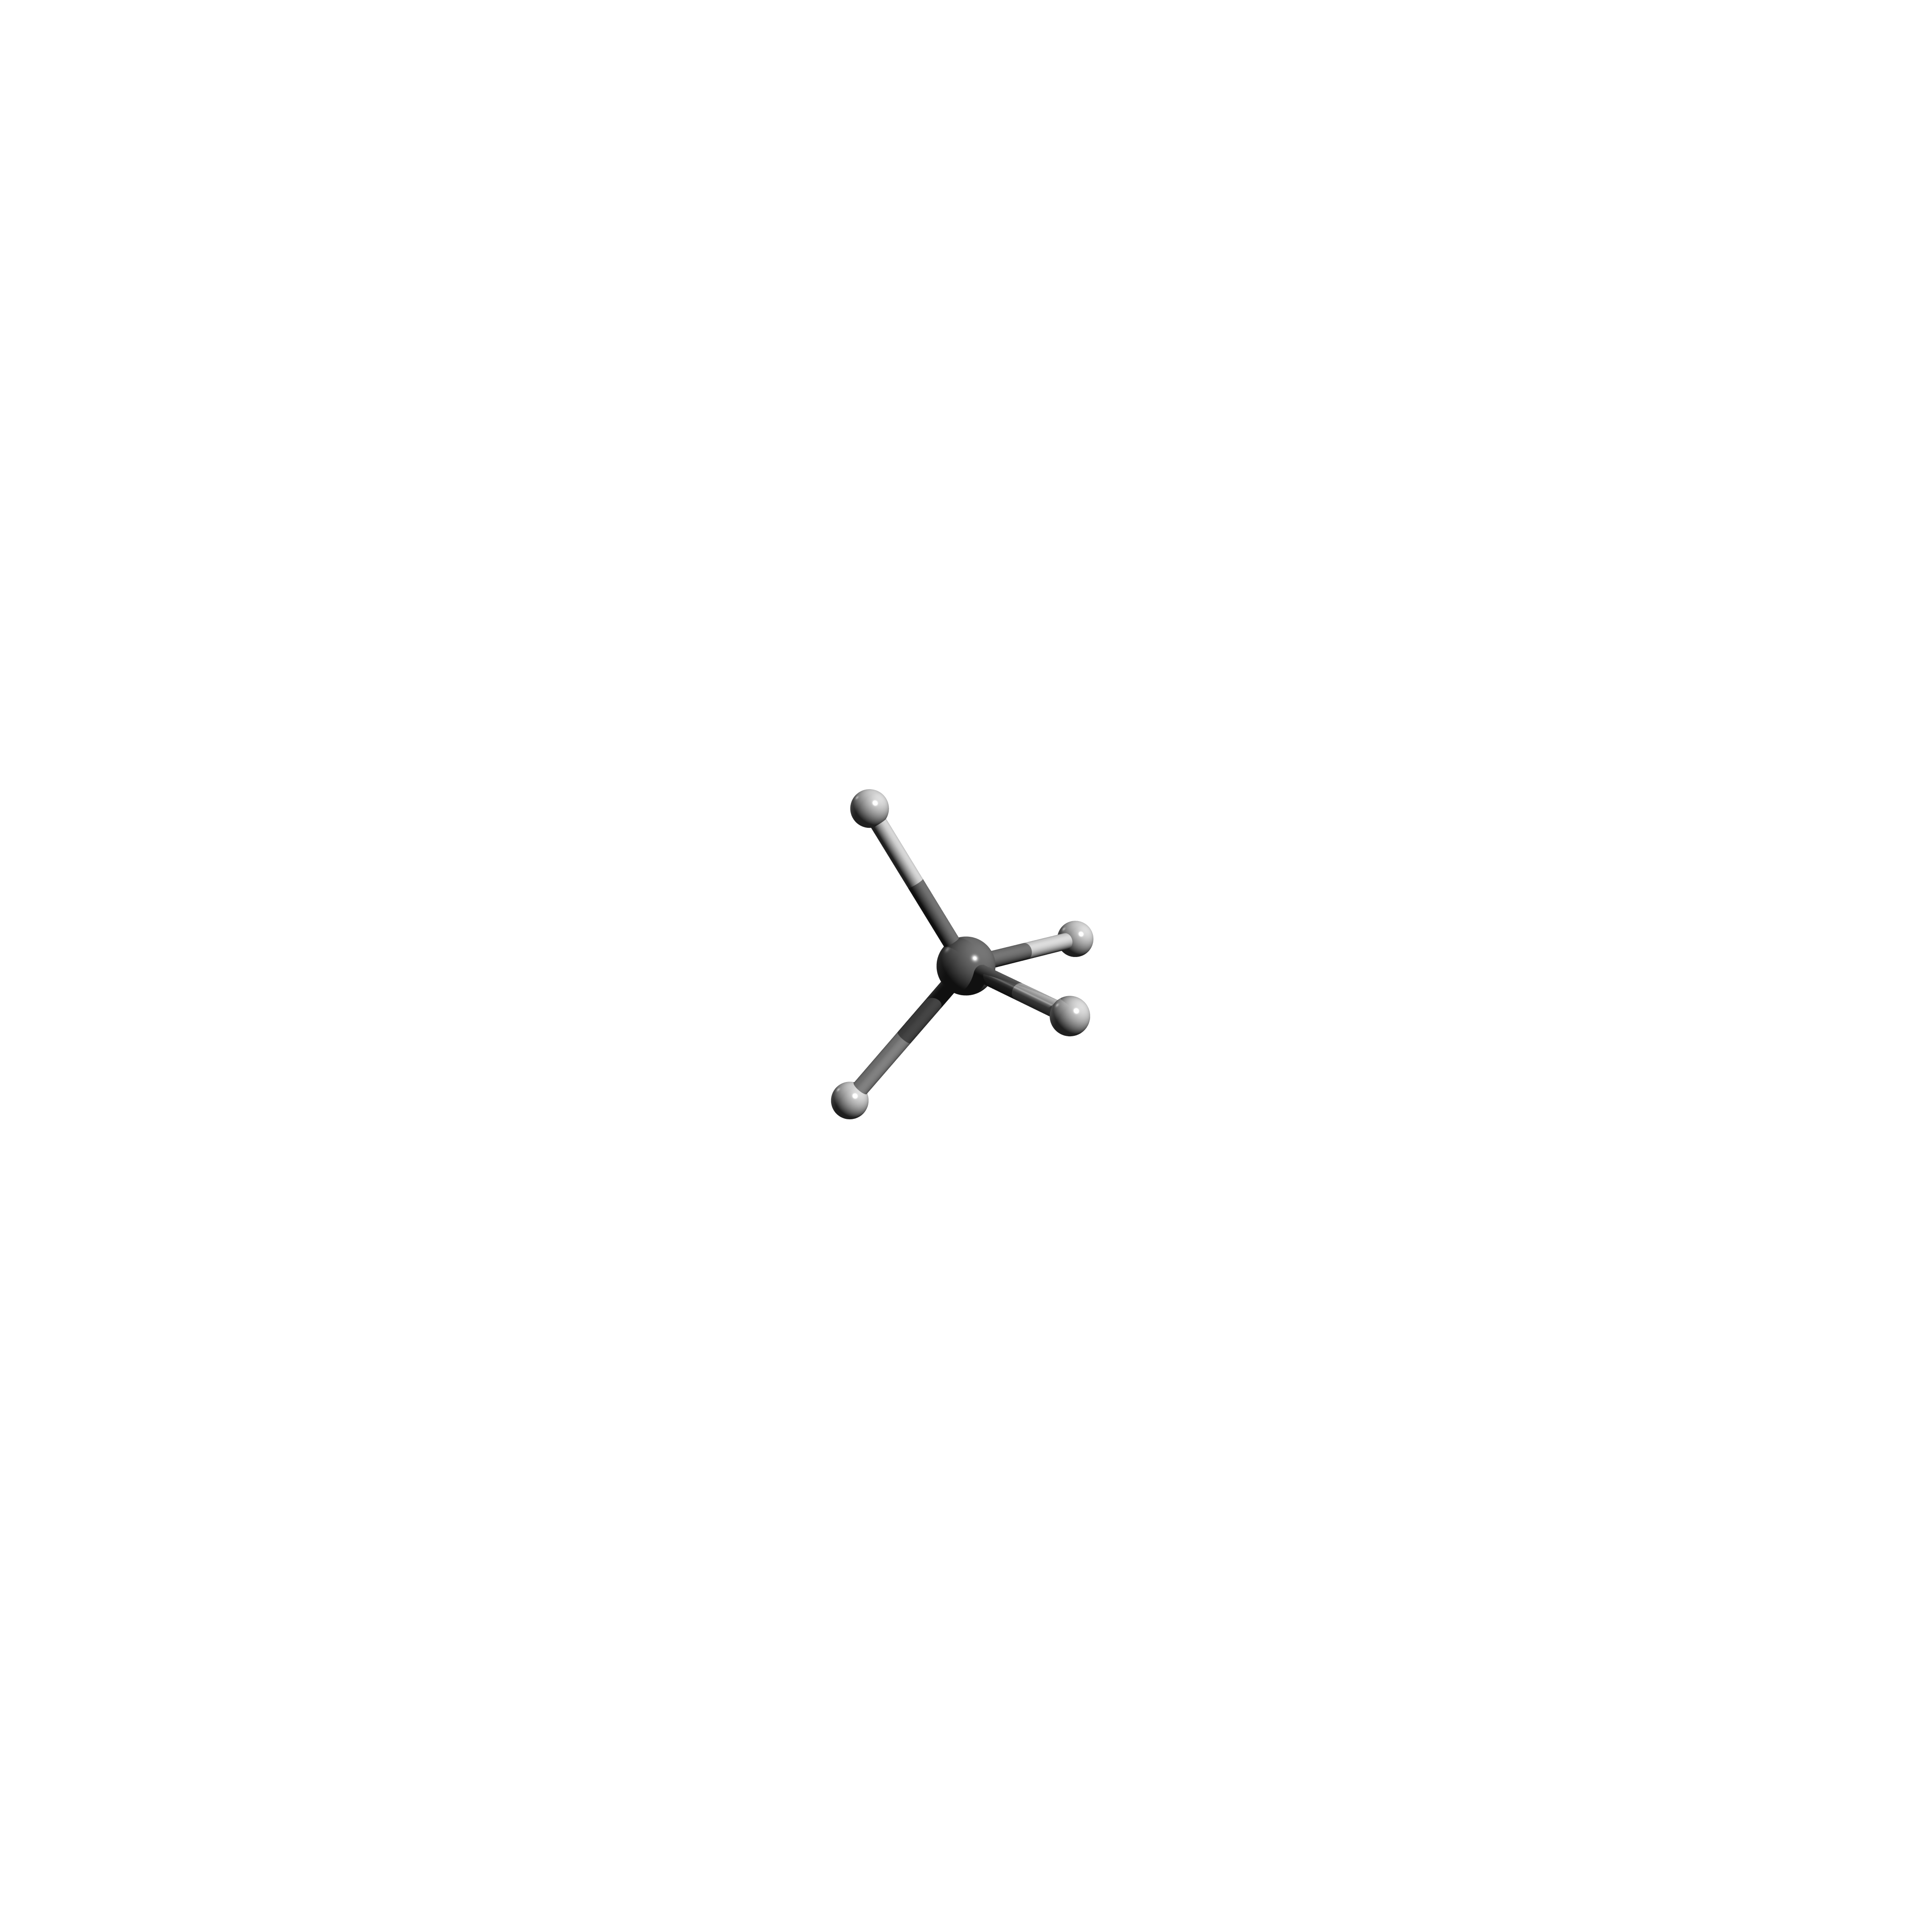
\includegraphics[trim=1400 1400 1400 1400, clip, width=0.24\textwidth]{res/CH4/ch4.png}
\caption{Von links nach rechts: HeH$^+$, H$_2$O, NH$_3$, CH$_4$}\label{molecules}
\end{figure}
Diese Moleküle sind verglichen zu
allen möglichen organischen Verbindungen
relativ einfache Konstrukte und dienen nur zum Testen
der grundlegenden Funktionalität.

Wir berechnen nun für jedes dieser Moleküle die Hartree\-/Fock\-/Energie, 
welche sich aus der elektronischen Energie und
der Internuklearen\-/Abstoßungs\-/Energie zusammen setzt.
Diese Energien vergleichen wir dann mit den
zuverlässigen Ergebnissen aus der NWChem\-/Software.
Es wird lediglich der 6-311+g** Basis\-/Satz verwendet,
dieser ist groß genug, um einigermaßen genaue Berechnungen zu ermöglichen.
Bei den Berechnungen wurden für möglichst identische Startbedingungen gesorgt.

\section{Numerische Experimente}
Diese Hartree\-/Fock\-/Energien (in Hartree) wurden berechnet:
\begin{center}
\begin{tabular}{c|c|c|c|c}
          & HeH$^+$ & H$_2$O & NH$_3$ & CH$_4$\\ \hline
    HFcpp & \unit[-2.88095]{Ha} & \unit[-73.88436]{Ha} & \unit[-54.55853]{Ha} & \unit[-39.01310]{Ha} \\
    NWChem & \unit[-2.92904]{Ha} & \unit[-76.04854]{Ha} & \unit[-56.21346]{Ha} & \unit[-40.20852]{Ha} \\ \hline
    Differenz & \unit[0.04809]{Ha} & \unit[2.16418]{Ha} & \unit[1.65493]{Ha} & \unit[1.19542]{Ha}\\
    Abweichung & $1.64\%$ & $2.85\%$ & $2.94\%$ & $2.97\%$
\end{tabular}
\end{center}

Wie klar zu erkennen ist, sind die berechneten Energien der eigenen Implementierung
im Bereich der Ergebnisse der NWChem\-/Software. Es lässt sich schlussfolgern,
dass die Implementierung korrekt ist.
Die deutlich besseren Ergebnisse der NWChem-Software
trotz gleicher Startbedingungen sind sehr wahrscheinlich 
auf Unterschiede in der Implementierung zurückzuführen,
wie zum Beispiel auf den Einsatz zusätzlicher Optimierungen.

Die Hartree\-/Fock\-/Energien sind jedoch nicht die einzigen Ergebnisse,
wir erhalten noch die Orbital\-/Funktionen und deren zugehörigen Energien.
Diese lassen sich in einem Isoflächen\-/Plot z.B. vom H$_2$O\-/Molekül gut darstellen:
\begin{figure}[h]
    \centering
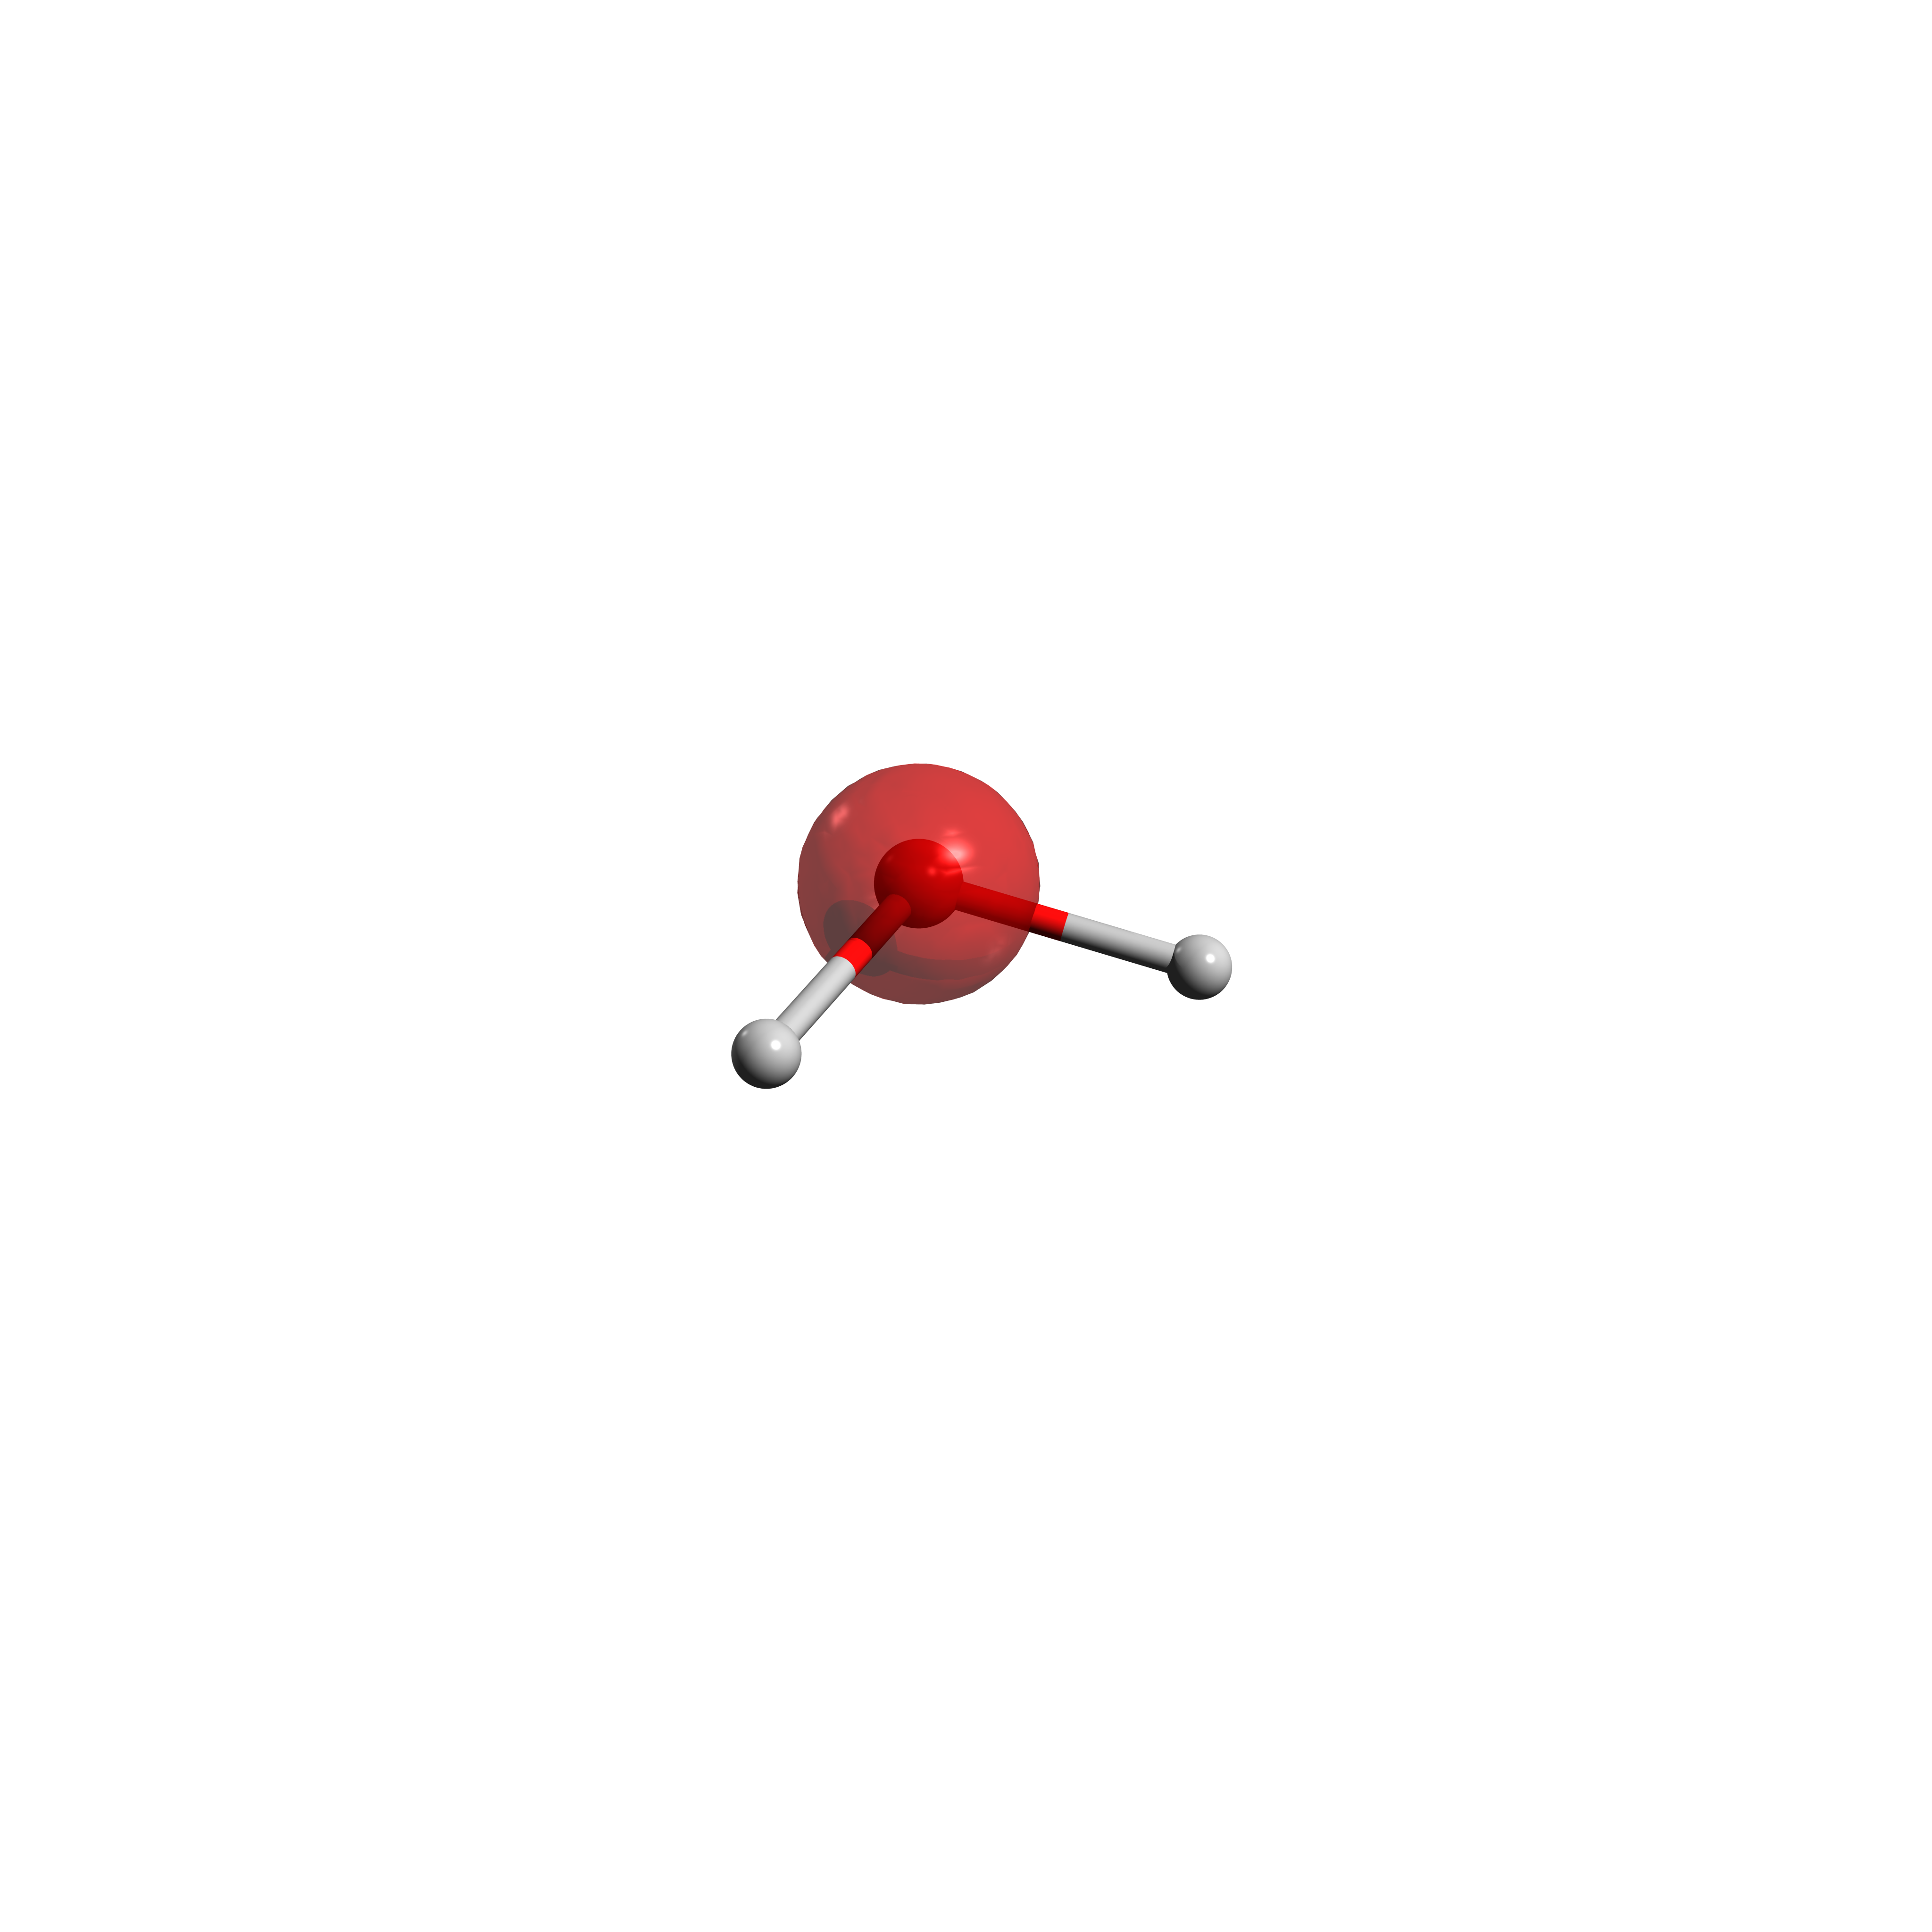
\includegraphics[trim=650 650 650 650, clip, width=0.32\textwidth]{res/H2O/h2o_w0.png}
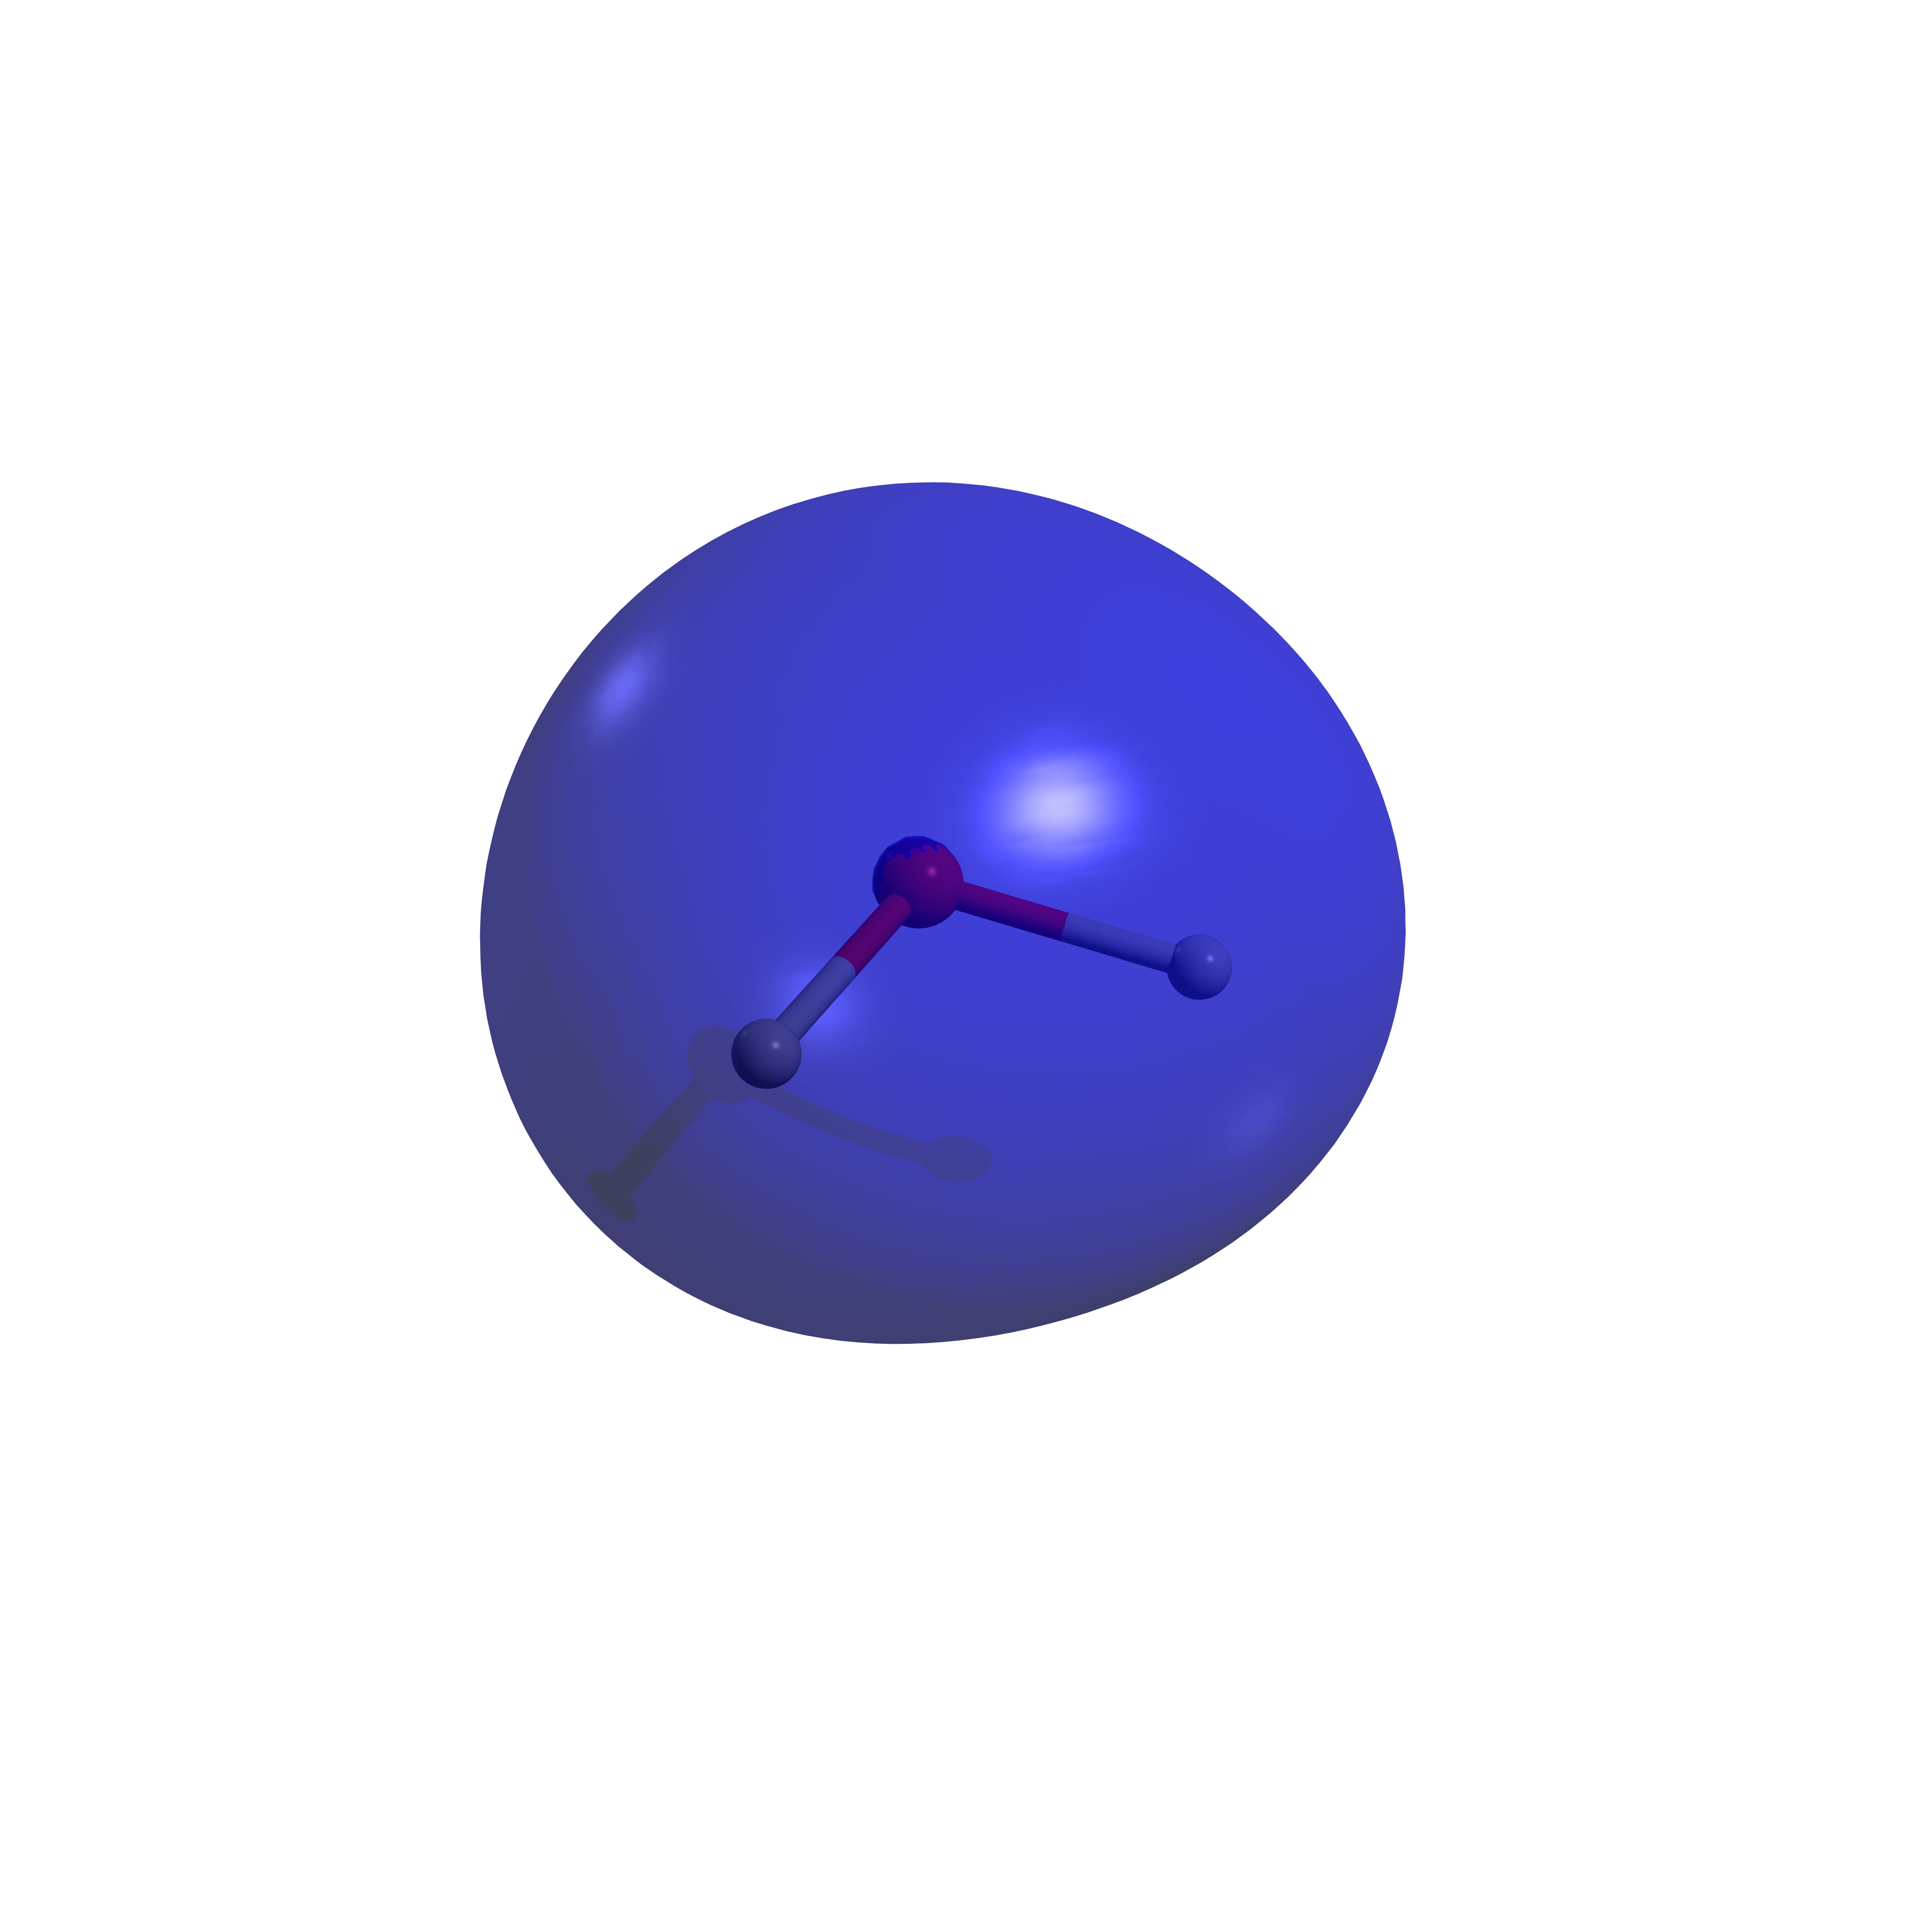
\includegraphics[trim=650 650 650 650, clip, width=0.32\textwidth]{res/H2O/h2o_w1.png}
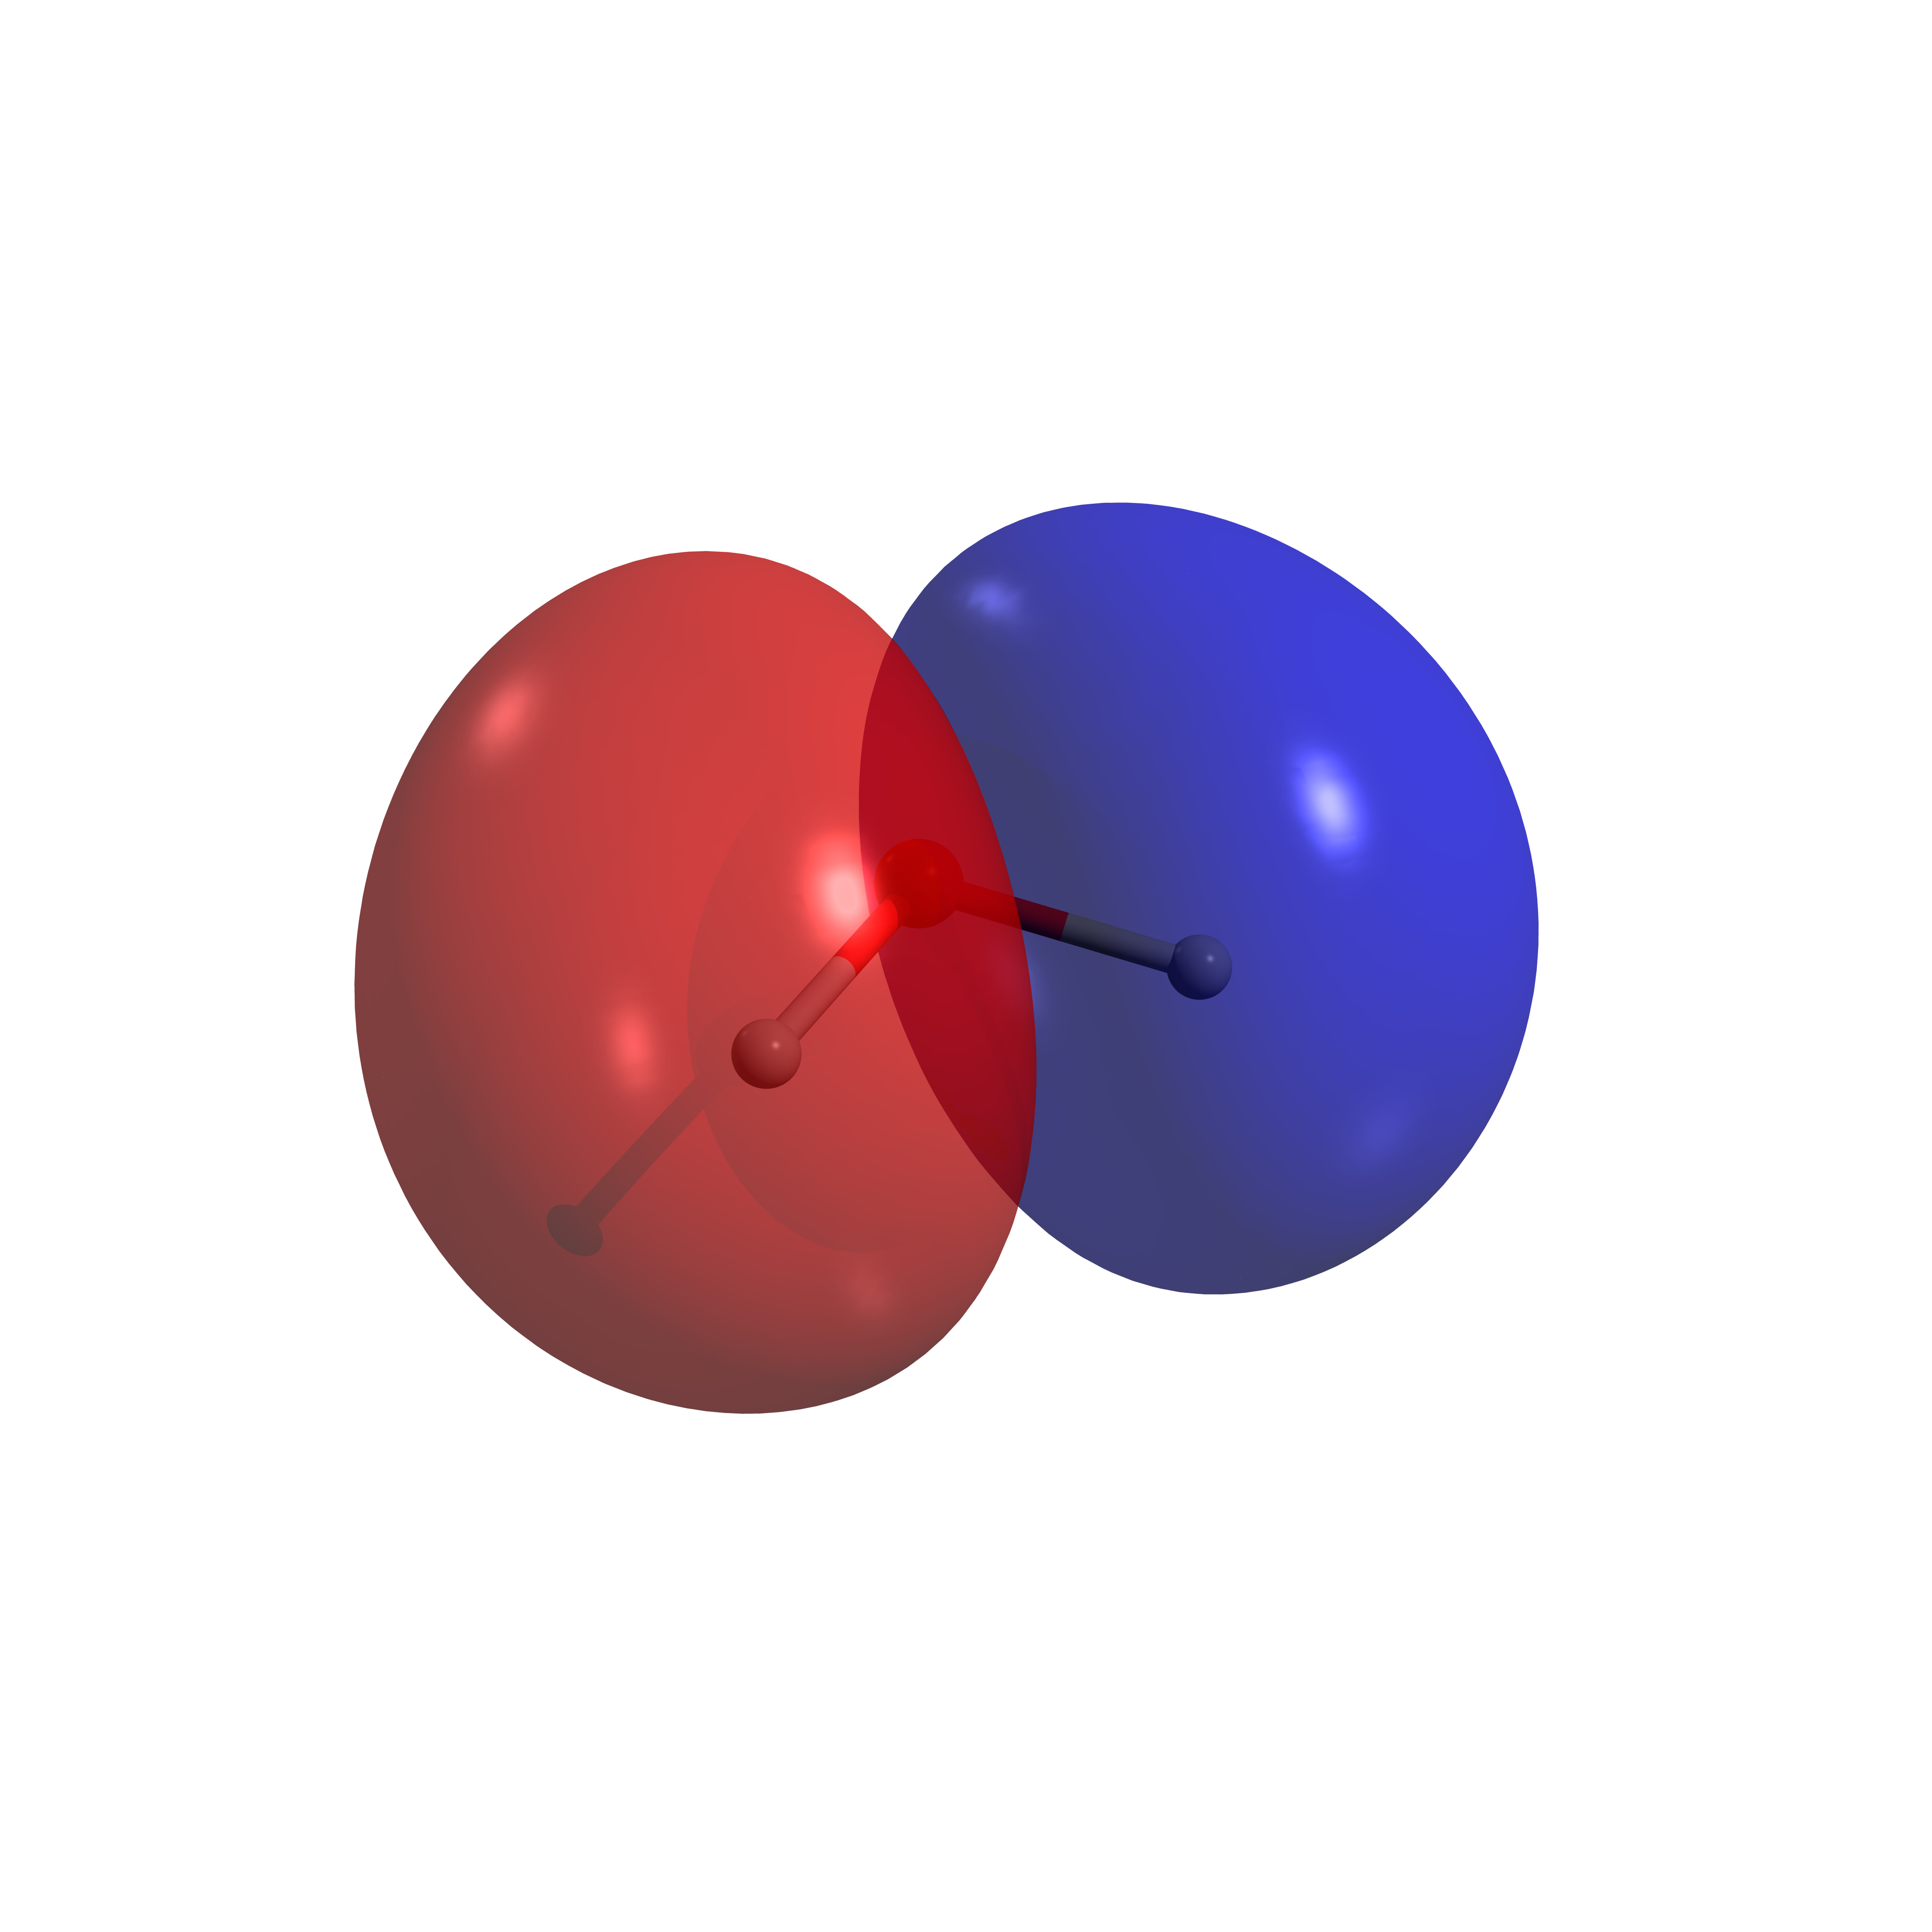
\includegraphics[trim=650 650 650 650, clip, width=0.32\textwidth]{res/H2O/h2o_w2.png}\\
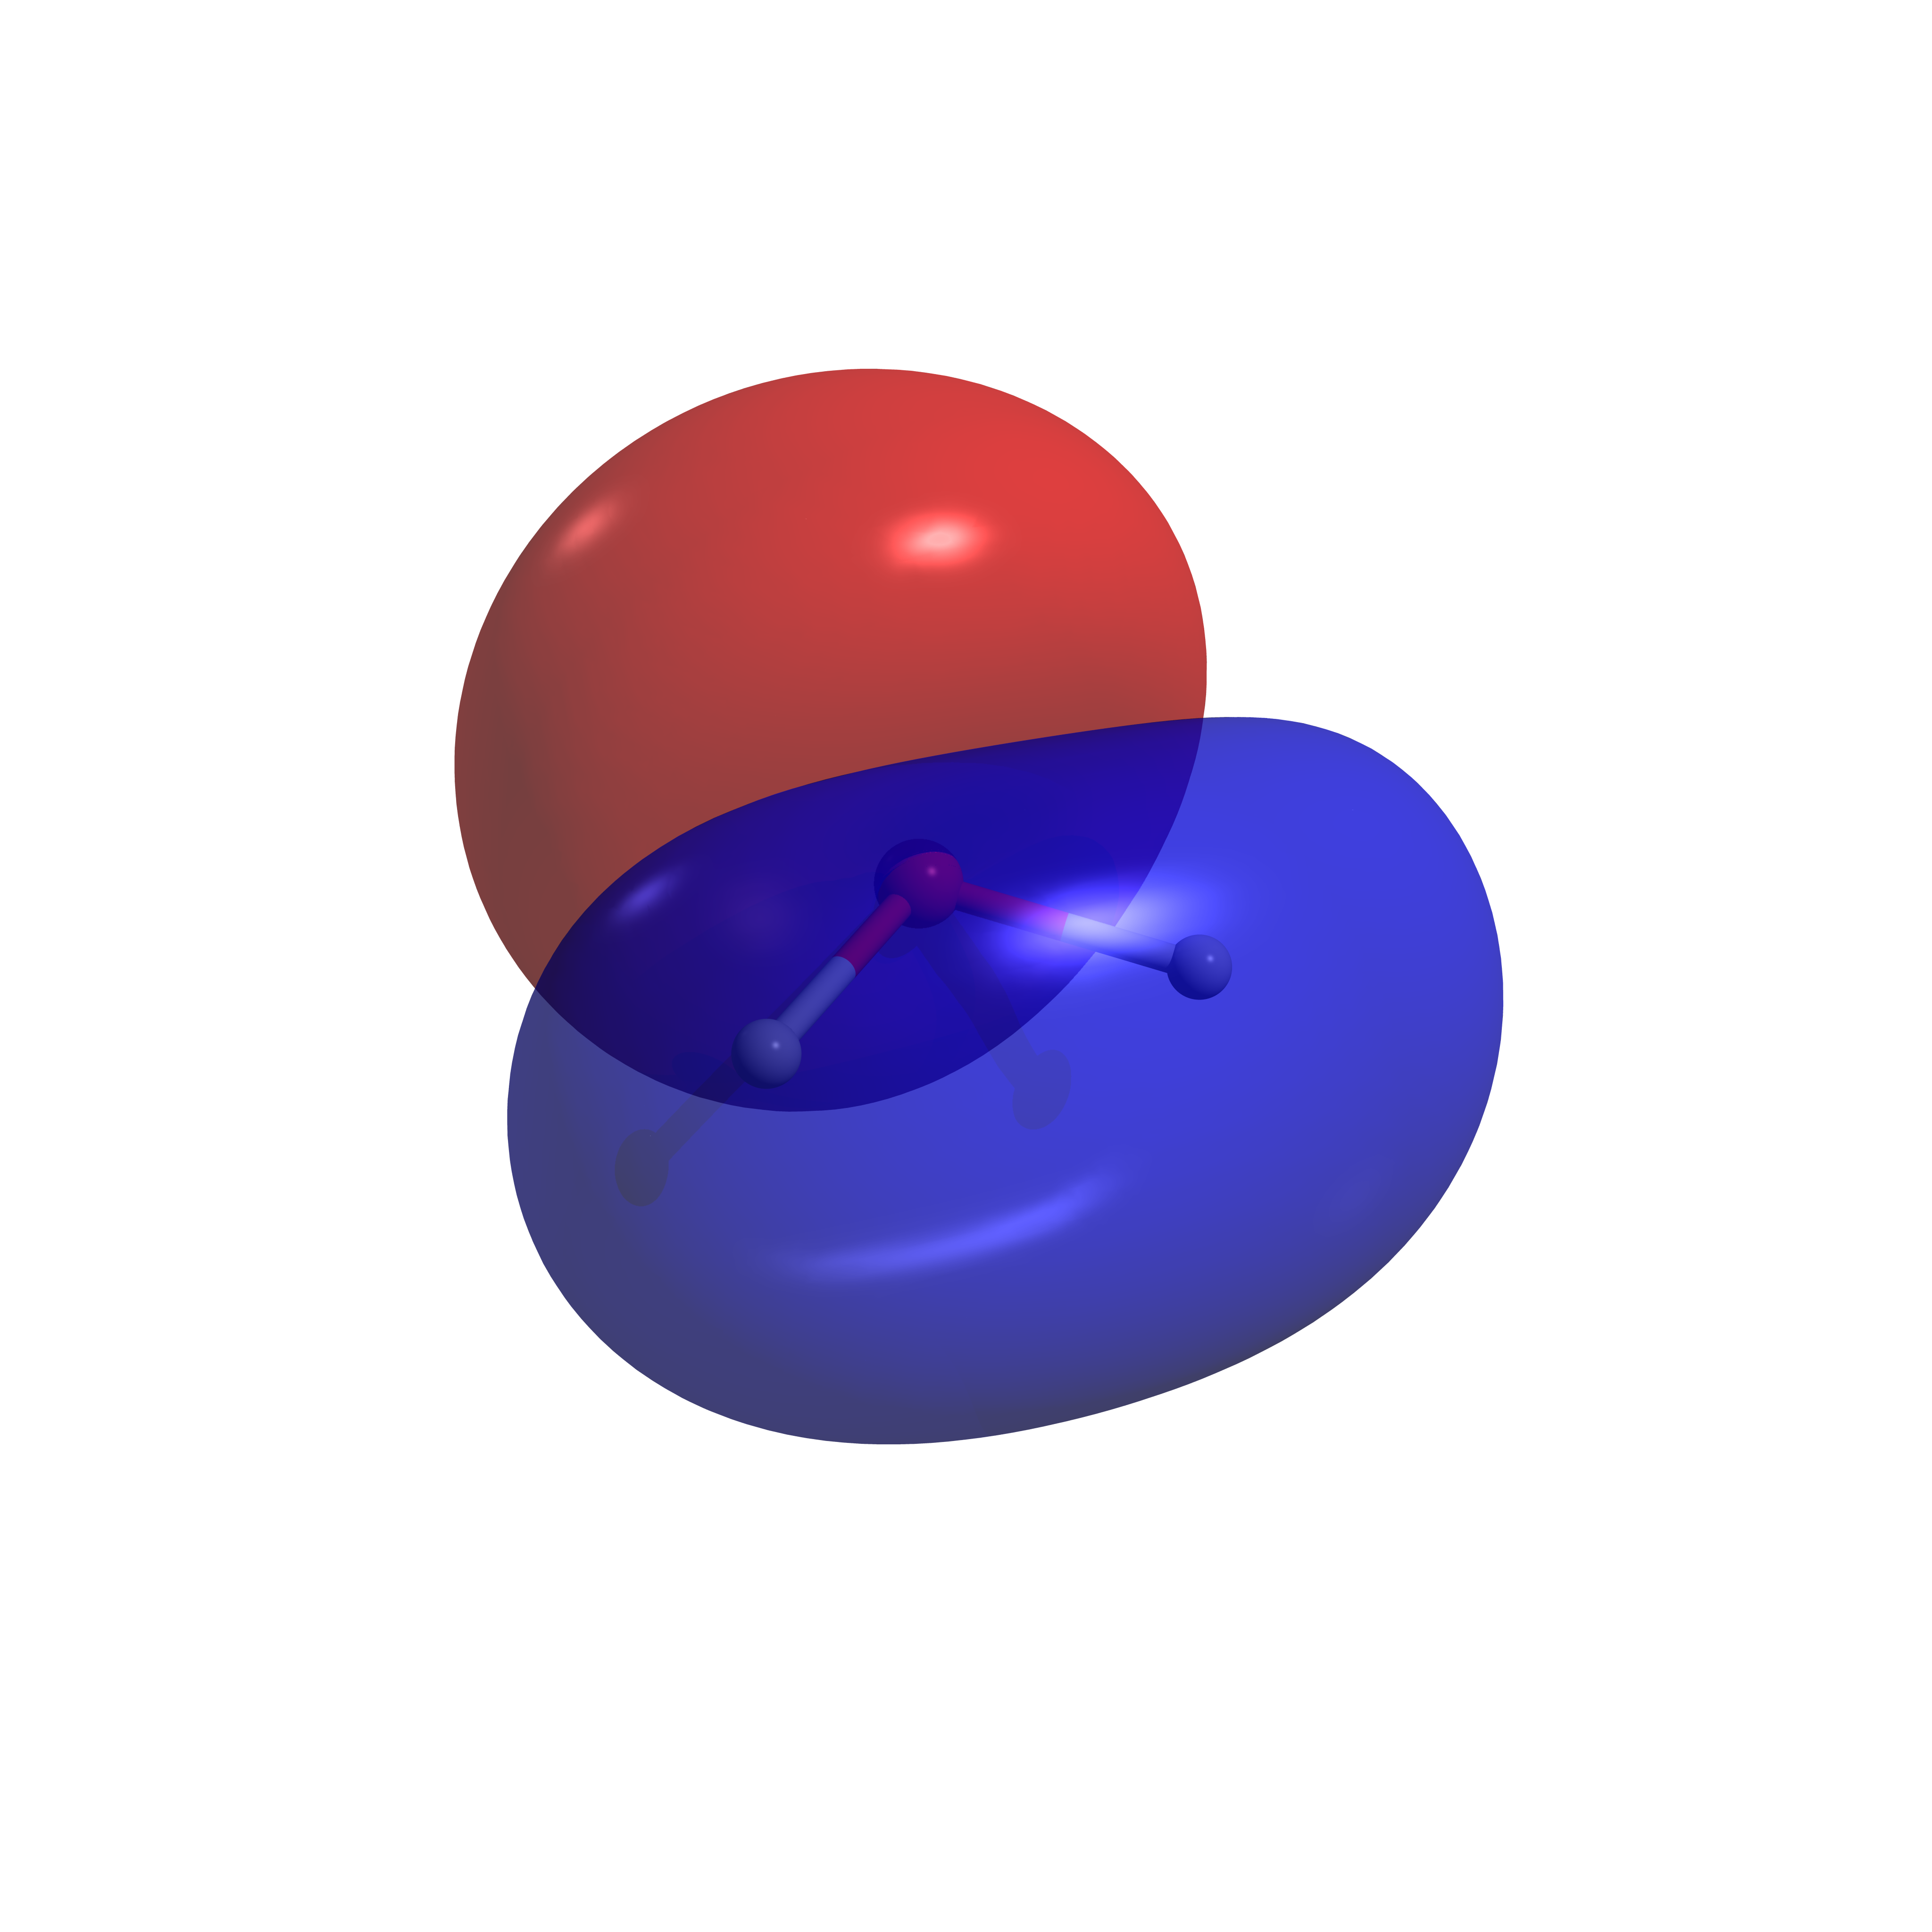
\includegraphics[trim=650 650 650 650, clip, width=0.32\textwidth]{res/H2O/h2o_w3.png}
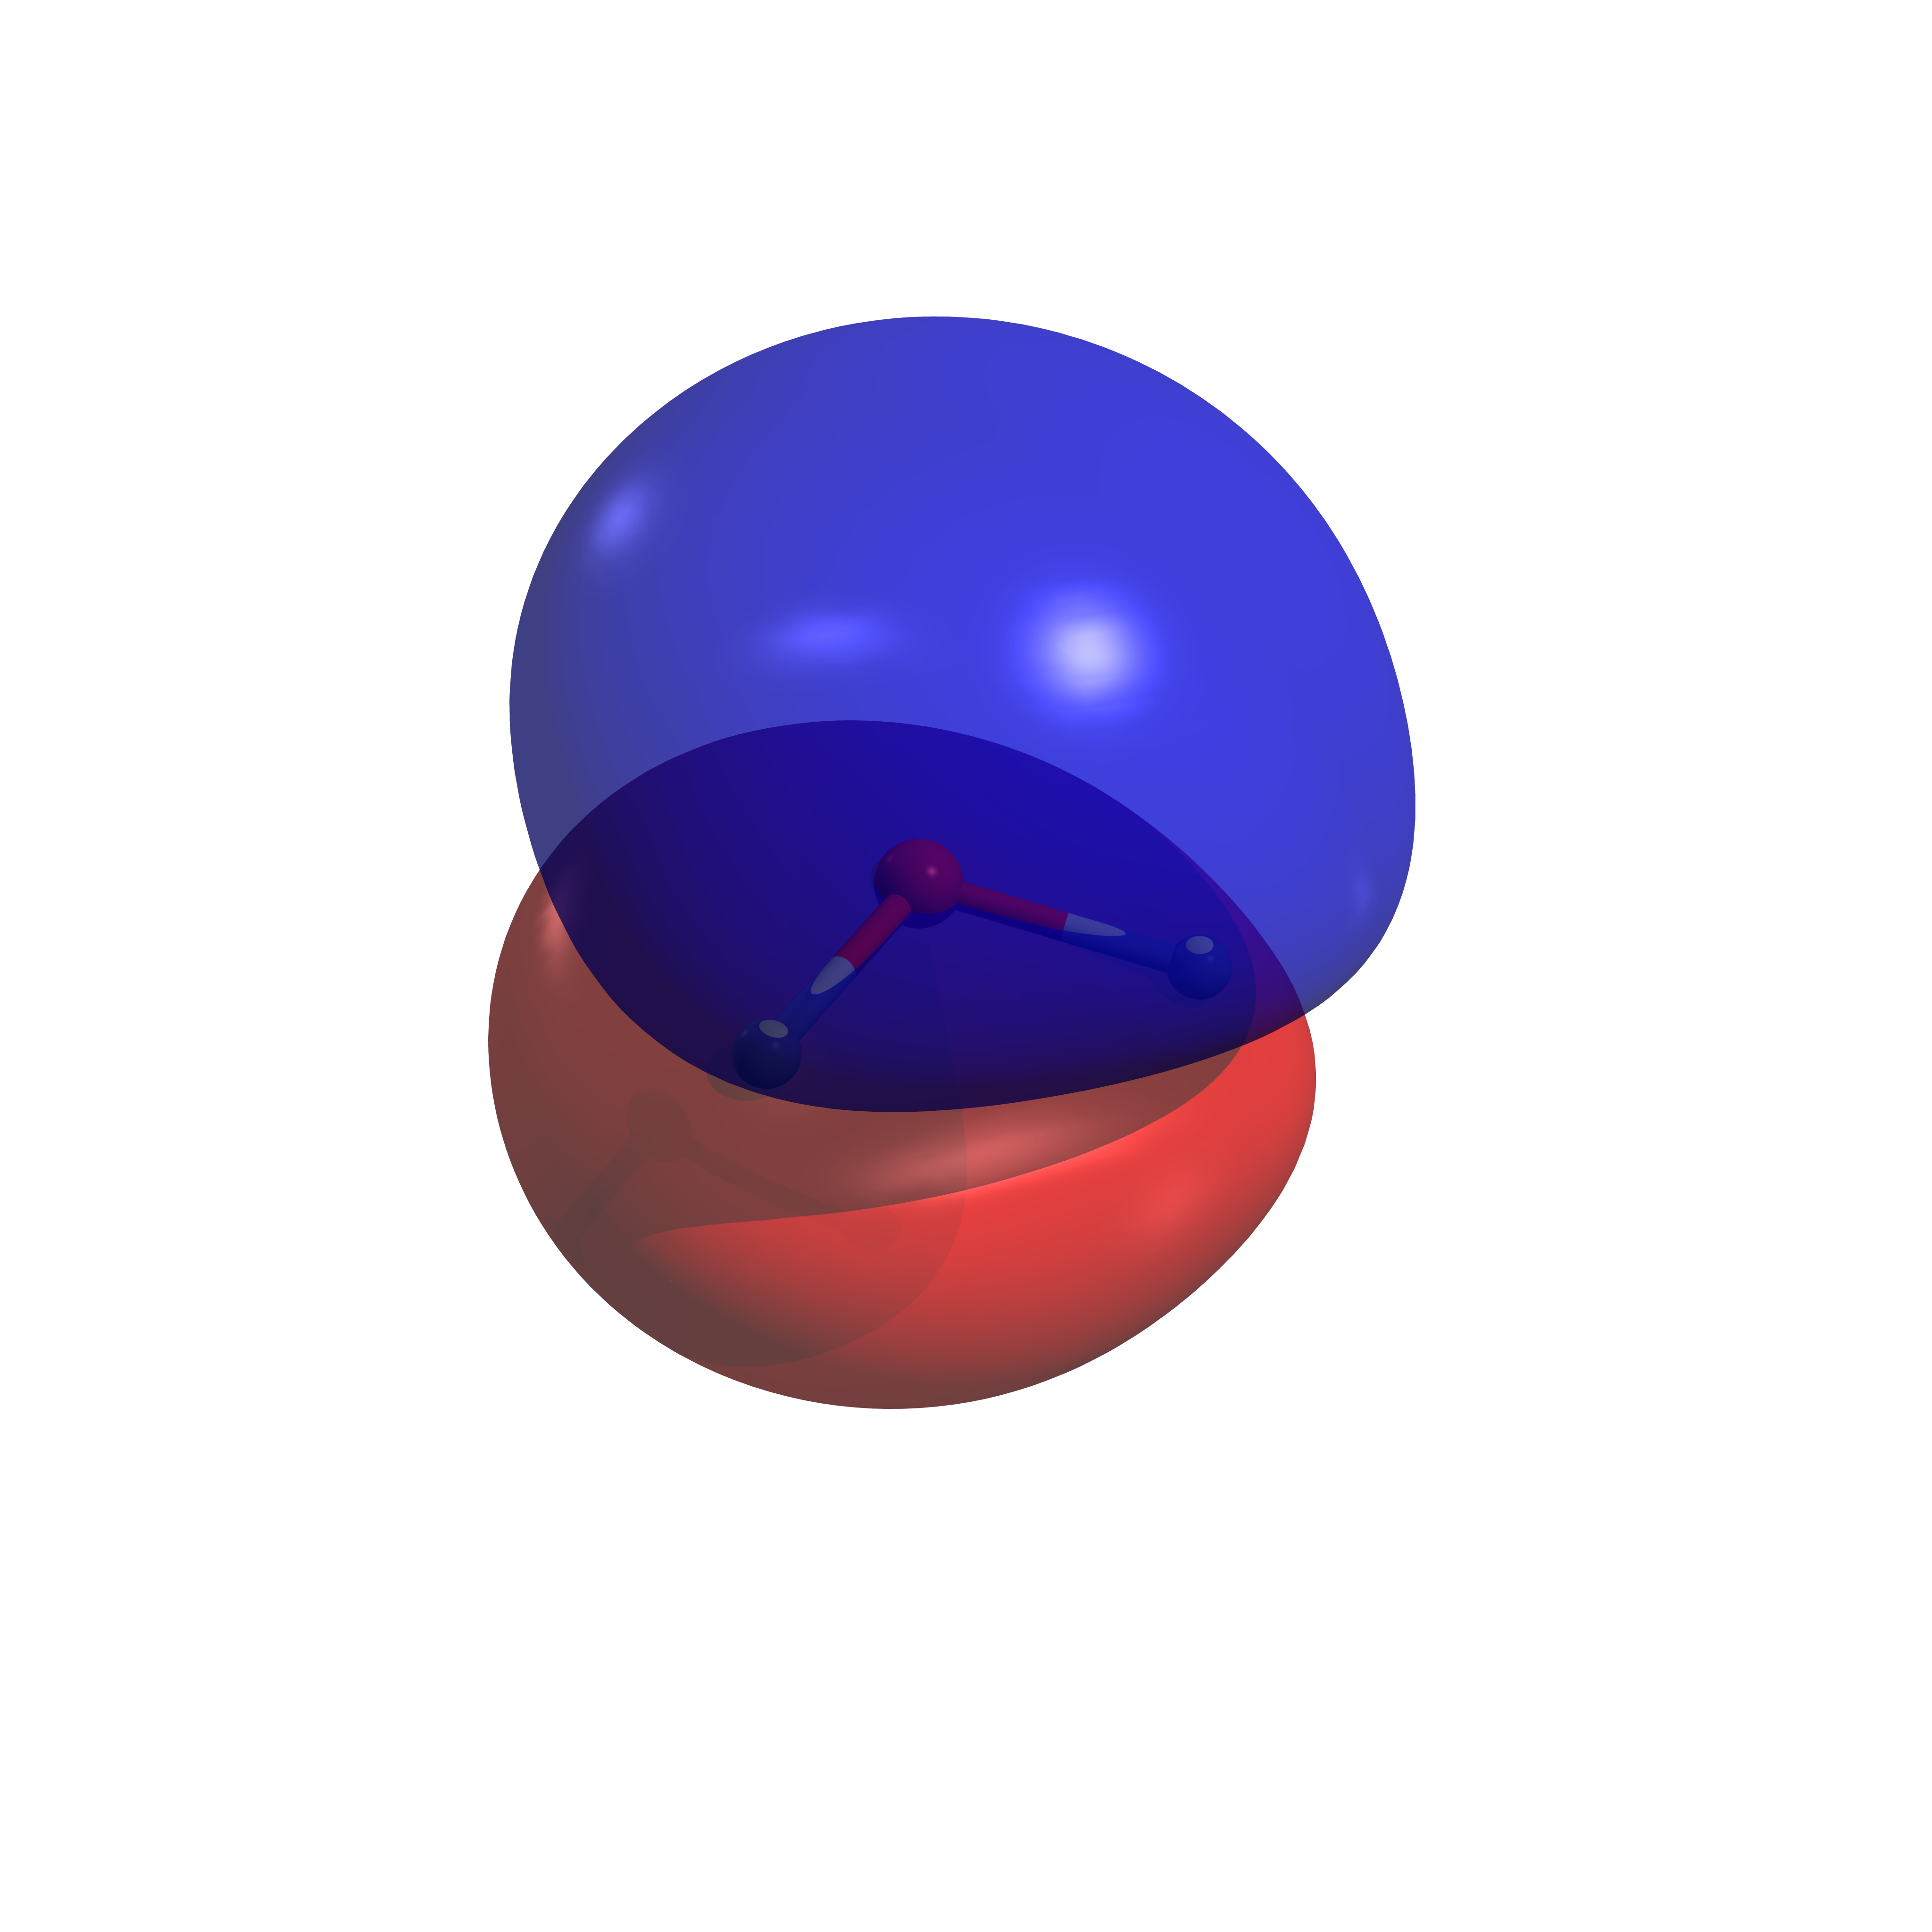
\includegraphics[trim=650 650 650 650, clip, width=0.32\textwidth]{res/H2O/h2o_w4.png}
\caption{Die fünf besetzten Orbitale des H$_2$O\-/Molekül,
nach aufsteigender Energie sortiert.
\textcolor{blue}{$\blacksquare$} positiv,
\textcolor{red}{$\blacksquare$} negativ.}\label{h2o_orbitals}
\end{figure}